\section{Wervelklokken en juiste tijd}

\begin{figure}[H]
    \centering
    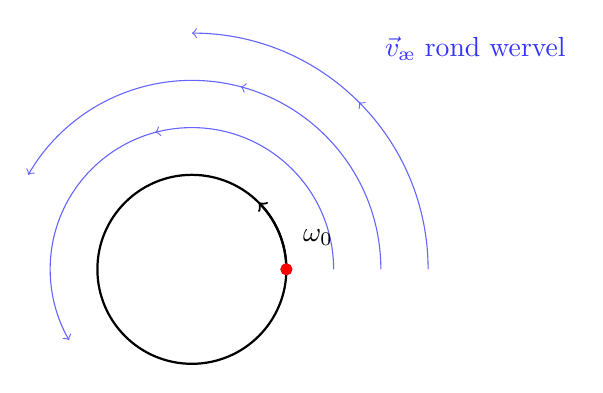
\begin{tikzpicture}[scale=2]
        \usetikzlibrary{decorations.markings}

        % Streamlines with varying arc lengths
        \draw[blue!60, ->,
            postaction={decorate},
            decoration={markings,
            mark=at position 0.5 with {\arrow{>}}}
        ] (0.9,0) arc (0:210:0.9); % Short arc

        \draw[blue!60, ->,
            postaction={decorate},
            decoration={markings,
            mark=at position 0.5 with {\arrow{>}}}
        ] (1.2,0) arc (0:150:1.2); % Medium arc

        \draw[blue!60, ->,
            postaction={decorate},
            decoration={markings,
            mark=at position 0.5 with {\arrow{>}}}
        ] (1.5,0) arc (0:90:1.5); % Long arc

        % Vortexring
        \draw[thick] (0,0) circle (0.6);
        \draw[thick, ->] (0:0.6) arc (0:45:0.6);
        \node at (0.8,0.2) {$\omega_0$};
        \filldraw[red] (0.6,0) circle (1pt);

        % Vectorveld label
        \node[blue!80] at (1.8,1.4) {$\vec{v}_{\ae}$ rond wervel};

    \end{tikzpicture}
    \caption{Elke $2\pi$ rotatie van de wervelkern = één tick van de interne klok.}
    \label{fig:wervelklok}
\end{figure}

In dit model wordt een klok gerealiseerd door de rotatie van een microscopische wervel. Om dit concreet te maken, beschouw een vrij deeltje in
rust in de æther. Zijn wervelkern draait gestaag en sleept de nabijgelegen æther rond. Laat $\omega_0$ de hoeksnelheid van deze kern  aanduiden, gemeten in het æther-rustframe (in eenheden radialen per seconde). Per definitie is $\omega_0$ de \emph{juiste rotatiefrequentie} van het deeltje, overeenkomend met zijn juiste tijd $\tau$.

We kunnen $\omega_0$ relateren aan het verstrijken van de juiste tijd: als de kern in een interval met $\Delta \theta$ radialen roteert, dan is de verstreken juiste tijd
\[
    \Delta \tau = \frac{\Delta \theta}{\omega_0} \,.
\]
Als we bijvoorbeeld $2\pi$ radialen van rotatie kiezen als een \("\)tik\("\) van de klok, dan is de juiste periode $T_0 = 2\pi/\omega_0$. Men zou zich kunnen voorstellen dat $\omega_0$ wordt bepaald door de interne structuur van het deeltje - bijvoorbeeld, de wervel van een proton zou kunnen roteren met ongeveer $10^{23}$ rad/s zodat $T_0 \sim 10^{-23}$ s voor één omwenteling (dit is speculatief, maar opmerkelijk genoeg stelde de Broglie in 1924 voor dat elk deeltje met rustmassa $m$ een interne klok heeft met frequentie $mc^2/h$~\cite{deBroglie1924-frequency}, in de orde van $10^{21}$ Hz voor een elektron; een wervelmodel zou een fysieke oorsprong kunnen bieden voor deze \emph{Zitterbewegung} frequentie als kernrotatie).

Voor nu is $\omega_0$ een vrije parameter die de kloksnelheid in rust weergeeft. Wanneer het deeltje niet vrij is of niet in rust is, kan de waargenomen rotatiesnelheid veranderen. We definiëren $\omega_{\textrm obs}$ als de hoeksnelheid van de wervelkern zoals waargenomen door een statische ætherframe-waarnemer (d.w.z. een in rust ten opzichte van de æther) onder welke omstandigheden dan ook (beweging of zwaartekracht). De verhouding $\omega_{\textrm obs}/\omega_0$ geeft dan de snelheid van de klok ten opzichte van de juiste tijd.

In feite, aangezien $\Delta \tau = \Delta \theta / \omega_0$ altijd geldt voor de klok zelf, en $\Delta t$ (coördinaattijd) overeenkomt met $\Delta \theta / \omega_{\textrm obs}$ (de hoek gedraaid in labframetijd), hebben we:
\[
    \frac{\Delta \tau}{\Delta t} = \frac{\Delta \theta / \omega_0}{\Delta \theta / \omega_{\textrm obs}} = \frac{\omega_{\textrm obs}}{\omega_0} \,. \tag{1}
\]

Deze belangrijke relatie koppelt de fysieke vertraging van de spin $\omega_{\textrm obs}$ van de wervel aan de tijdsdilatatiefactor. Als $\omega_{\textrm obs} < \omega_0$, loopt de klok langzaam (aangezien $\Delta \tau < \Delta t$).

Onze taak in de volgende secties is om $\omega_{\textrm obs}$ te bepalen voor twee gevallen:
\begin{enumerate}
    \item Wanneer de wervel (deeltje) met snelheid $v$ door de æther beweegt,
    \item Wanneer de wervel zich in een gravitatiepotentiaal (ætherstroom) bevindt die wordt gecreëerd door een massief lichaam.
\end{enumerate}
We zullen ontdekken dat $\omega_{\textrm obs}/\omega_0$ in deze gevallen respectievelijk de bekende Lorentz- en gravitationele tijdsdilatatiefactoren reproduceert.

Voordat we verdergaan, benadrukken we dat \emph{eigen tijd $\tau$ in dit model fundamenteel slechts een telling is van de rotatie van de wervel}. Dit biedt een objectief, mechanistisch beeld van tijd: bijvoorbeeld, je zou je een klein vlaggetje of markering op de wervelkern kunnen voorstellen die rondjes rond de kern voltooit – elke ronde is een ondubbelzinnige fysieke gebeurtenis die overeenkomt met een vaste hoeveelheid eigen tijd. Verschillende fysieke klokken (atomen, moleculen, etc.) zouden uiteindelijk allemaal hun tijd traceren naar zulke microscopische circulaties in de universele æther.

Voor een bespreking van hoe samengestelde klokken bestaande uit meerdere wervelknopen collectief tijdsdilatatie ondervinden, zie Appendix~\ref{appendix:KlokkenInWervelstructuren}.

Zolang de natuurkundige wetten zodanig zijn dat deze circulaties stabiel en identiek zijn voor identieke deeltjes, biedt dit een standaard van tijd. Vervolgens laten we zien hoe beweging door de æther en ætherstromen $\omega_{\textrm obs}$ beïnvloeden.